% ACL-style submission. Compile with the official ACL template (acl.sty + acl_natbib.bst):
%   Overleaf: start from the "ACL Rolling Review" template; upload main.tex, references.bib and figures/.
%   Local:    put acl.sty and acl_natbib.bst from https://github.com/acl-org/acl-style-files next to this file,
%             then  pdflatex main && bibtex main && pdflatex main && pdflatex main
\documentclass[11pt]{article}
\usepackage[review]{acl}
\usepackage{times}
\usepackage{latexsym}
\usepackage[T1]{fontenc}
\usepackage[utf8]{inputenc}
\usepackage{microtype}
\usepackage{inconsolata}
\usepackage{graphicx}
\usepackage{booktabs}
\usepackage{multirow}
\usepackage{amsmath}
\usepackage{amssymb}
\usepackage{xcolor}
\usepackage{tikz}
\usetikzlibrary{positioning,arrows.meta}

\newcommand{\SB}{\textsc{SB}}
\newcommand{\SDB}{\textsc{SD-B}}
\newcommand{\SDC}{\textsc{SD-C}}
\newcommand{\Dense}{\textsc{D270}}
\newcommand{\PLD}{\textsc{PLD}}
\newcommand{\Lngram}{\textsc{Lngram}}
\newcommand{\ci}[2]{\,{\scriptstyle[#1,\,#2]}}  % use inside math mode

\title{Self-Drafting Latent Memory: What an $n$-gram Memory Learns,\\and When It Can Draft for Its Own Model}

\author{Anonymous ACL submission}

\begin{document}
\maketitle

\begin{abstract}
Route $n$-gram memories such as \Lngram{} attach a large lookup table to a transformer. A router turns each position
into a few discrete codes, and the codes of the last few positions select rows of the table. Because rows are selected
by codes rather than by dense activations, a memory whose codes depend only on tokens could read its own table
\emph{without running the model}. That makes it a built-in drafter for speculative decoding. We study this idea in 370M-parameter
language models trained on 1B tokens.

We find that \textbf{self-drafting is free}. Making the router token-only and training a draft head jointly changes
validation loss by $+0.0004$ to $+0.003$ nats, within the 0.002-nat difference between two training runs of the baseline,
and leaves six zero-shot benchmarks unchanged. It is free because \textbf{layer-1 routing is already a near per-token
lookup}: the current token explains 86\% of the baseline's code entropy, and codes predicted from three tokens retain 99.8\%
of the memory's 0.28-nat contribution. \textbf{Joint training makes a far better drafter than post-hoc fitting}: top-1
agreement rises from 0.30 to 0.45 and accepted length roughly doubles. A small diagonal SSM adds 25--30\%, and next-token
counts keyed by the model's own codes reach 2.5--2.6 accepted tokens per step.

Interpretability analyses explain when self-drafting helps. Prompt lookup's lead comes from greedy self-repetition:
49\% of continuation tokens copy the model's own output. Before repetition sets in, the self-drafting heads accept
40--65\% more than prompt lookup. A hybrid of the two beats prompt lookup on every model and text type, and the drafter's
own confidence identifies where it is reliable (88\% agreement at a 0.5 threshold). The memory's codes form emergent
word-class partitions that are not unique across training runs, and the memory specialises in frequent, local and
formatting tokens. Serving the table from host memory is bit-exact at ${\sim}1\%$ latency cost. We release all code, logs
and results.
\end{abstract}

%=====================================================================
\section{Introduction}
%=====================================================================

Speculative decoding \citep{leviathan2023fast,chen2023accelerating} accelerates generation by letting a cheap
\emph{drafter} propose $\gamma$ tokens that the target model verifies in a single forward pass. Drafters range from small
language models and extra decoding heads \citep{stern2018blockwise,cai2024medusa,li2024eagle} to model-free retrieval
from the prompt or a datastore \citep{saxena2023pld,he2024rest,fu2024lookahead}. Model-based drafters are accurate but
need the target's hidden states or a second network. Retrieval drafters are almost free but know nothing about the
target.

Large \emph{memory layers} \citep{lample2019pkm,berges2024memory} suggest a third kind of drafter. A route $n$-gram memory
\citep[\Lngram;][]{lngram} quantises a vector into $R$ short codes per position. For each route, the codes of the last $n$
positions address a row of a large table, and an attention readout mixes the retrieved rows into the residual stream.
Rows are selected by \emph{discrete codes}. If the codes depended only on tokens, a drafter could compute them, read the
same rows, and propose tokens without touching the backbone. In speculative decoding, the rows for a drafted block
could even be staged from host memory before verification. The table would then provide model capacity and a drafter
at once. We call this \emph{self-drafting latent memory}.

We ask:
\textbf{(RQ1)} What does making a memory self-drafting cost the language model?
\textbf{(RQ2)} How predictable are memory codes from tokens, and why?
\textbf{(RQ3)} How well can the memory draft, and how does a jointly trained drafter compare with post-hoc and
model-free drafters?
\textbf{(RQ4)} What do these memories learn, and what does that imply for when self-drafting pays off?

\paragraph{Contributions.}
\begin{itemize}
\setlength\itemsep{1pt}
\item \textbf{A self-drafting memory design} (\S\ref{sec:method}): token-only routing, optionally with a diagonal SSM
for document context; a backbone-free draft readout trained by stop-gradient distillation; code-keyed online counts; and
a serving layout that makes next-step candidate rows contiguous.
\item \textbf{Self-drafting is free, and we explain why} (\S\ref{sec:cost}, \S\ref{sec:why}). There is no measurable cost in loss or downstream
accuracy, because layer-1 routing is already almost a per-token lookup. Substituting token-predicted codes keeps 99.8\% of the memory's value.
\item \textbf{Joint training makes a much better memory drafter} than post-hoc fitting: 0.45 vs.\ 0.30 top-1 agreement, and
about twice the accepted length (\S\ref{sec:drafting}).
\item \textbf{When drafting helps} (\S\ref{sec:when}). Prompt lookup wins through greedy self-repetition, while learned
heads win before it begins. A hybrid drafter beats prompt lookup everywhere, and the drafter's own confidence is a reliable
gate.
\item \textbf{What the memory learns} (\S\ref{sec:learn}): emergent word-class codes, non-identifiable code
assignments, route redundancy under hidden-state routing, and specialisation in frequent, local and formatting tokens.
\item \textbf{Exact host-memory serving} and a full open release of code, logs and results (\S\ref{sec:serving}).
\end{itemize}

%=====================================================================
\section{Background}
\label{sec:background}
%=====================================================================

\paragraph{Route $n$-gram memory.}
We use \Lngram{} v2 \citep{lngram}. At position $t$, a router produces $R\cdot b$ logits ($b{=}4$). Their signs give $R$
codes $c_r[t]\in\{0,\dots,15\}$. For each order $n\in\{2,3\}$ and route $r$, the codes $c_r[t-n+1..t]$ address one row of an
order-$n$ table with $R\cdot16^n$ rows of dimension 128. The two rows of a route are concatenated into a 256-d \emph{route
token}, RMS-normalised \citep{zhang2019rmsnorm} and projected to keys and values (4 KV heads $\times$ 64). A query from the
hidden state (16 heads) attends over the $R$ route tokens together with a fixed, zero-valued \emph{sink} of logit
$b_0=\log(R(1-m)/m)$, $m{=}0.5$. A depthwise causal convolution follows the output projection. The router is trained
through a one-bit counterfactual surrogate gradient, in the spirit of straight-through estimators
\citep{bengio2013estimating}.

\paragraph{Speculative decoding.}
Under greedy verification, a drafter proposes $\gamma$ tokens and the target accepts the longest prefix that matches its
own greedy choices, plus one token of its own \citep{leviathan2023fast}. With $A$ accepted tokens per step and a drafting
cost of $c$ target-steps per token, the speedup is approximately $\mathbb{E}[A{+}1]/(1+\gamma c)$, when a verification step
costs about one decoding step.

%=====================================================================
\section{Self-Drafting Latent Memory}
\label{sec:method}
%=====================================================================

\begin{figure}[t]
\centering
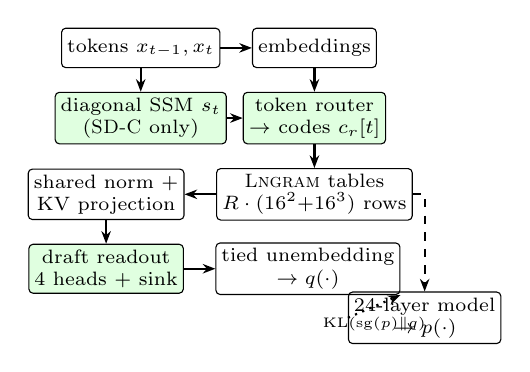
\begin{tikzpicture}[font=\scriptsize, node distance=3mm and 4mm,
  box/.style={draw, rounded corners=1.5pt, minimum height=5mm, align=center, inner sep=2pt},
  hl/.style={box, fill=green!12},
  ar/.style={-{Stealth[length=1.6mm]}, thick}]
\node[box] (tok) {tokens $x_{t-1}, x_t$};
\node[box, right=of tok] (emb) {embeddings};
\node[hl, below=of tok] (ssm) {diagonal SSM $s_t$\\(\SDC{} only)};
\node[hl, below=of emb] (router) {token router\\$\to$ codes $c_r[t]$};
\node[box, below=of router] (table) {\Lngram{} tables\\$R\cdot(16^2{+}16^3)$ rows};
\node[box, left=of table] (kv) {shared norm +\\KV projection};
\node[hl, below=of kv] (draft) {draft readout\\4 heads + sink};
\node[box, right=of draft] (unemb) {tied unembedding\\$\to q(\cdot)$};
\node[box, below=of table, xshift=14mm, yshift=-6mm] (backbone) {24-layer model\\$\to p(\cdot)$};
\draw[ar] (tok) -- (emb);
\draw[ar] (emb) -- (router);
\draw[ar] (tok) -- (ssm);
\draw[ar] (ssm) -- (router);
\draw[ar] (router) -- (table);
\draw[ar] (table) -- (kv);
\draw[ar] (kv) -- (draft);
\draw[ar] (draft) -- (unemb);
\draw[ar, dashed] (table.east) -| (backbone.north);
\draw[ar, dotted] (backbone.west) -- node[below, font=\tiny]{KL$(\mathrm{sg}(p)\Vert q)$} (unemb.south east);
\end{tikzpicture}
\caption{Self-drafting memory. The router reads token embeddings (plus an SSM state in \SDC), so codes and rows can be
computed without the backbone. A draft head reads the same rows through the memory's shared KV projection and is
distilled from the model's own stop-gradient distribution.}
\label{fig:arch}
\end{figure}

\paragraph{Token-only routing.}
Instead of the block's hidden state, the router reads $[\mathrm{RMSNorm}(E[x_{t-1}]);\mathrm{RMSNorm}(E[x_t])]$, with a
learned start vector at $t{=}0$. \SDC{} appends the state $s_t$ of a non-selective diagonal SSM \citep{gupta2022dss}:
$u_t = W_{\text{in}}\,\mathrm{RMSNorm}(E[x_t])$ and $s_t=a\odot s_{t-1}+(1-a)\odot u_t$, with 256 channels and decays
$a=\sigma(\theta)$ initialised geometrically in $[0.5,0.999]$. Training uses a chunked parallel scan in fp32, and decoding
uses the recurrence. \SDB{}'s codes are an exact function of $(x_{t-1},x_t)$, and \SDC{}'s depend on the prefix only
through $s_t$. Neither ever depends on backbone activations.

\paragraph{Backbone-free draft readout.}
For position $t$, the draft head takes the route tokens that the memory layer reads. It passes them through the memory's
\emph{shared} norm and KV projection and attends over them with 4 query heads (dimension 64), using the same sink-augmented
softmax. The query is $W_q\,\mathrm{RMSNorm}(E[x_t])$, plus $W_{sq}s_t$ in \SDC. The output is projected to $d$, normalised,
and scored against the tied embedding matrix. The head adds only 0.53M parameters (0.59M with the SSM query). A unit test
randomises every backbone weight and checks that draft logits are bitwise unchanged.

\paragraph{Joint objective.}
We train with $\mathcal{L}=\mathcal{L}_{\text{LM}}+\lambda\,\mathrm{KL}(\mathrm{sg}(p)\Vert q)$, $\lambda=0.1$, where $p$
is the model's next-token distribution and $q$ the draft distribution
\citep{hinton2015distilling,zhou2024distillspec}. The KL term uses a random 25\% of positions per sequence, seeded by step
and sequence id so that it is independent of hardware layout, in fp32 chunks of 512 positions. The draft path sees
embeddings only through detached copies. Its gradients therefore reach the tables, the KV projection, the router (via
the surrogate) and the SSM, but never attention, the FFNs or the embeddings. We verify this with gradient tests.
Self-drafting models drop routes until their non-embedding size matches the baseline within 0.05\% (Table~\ref{tab:models}).

\paragraph{Post-hoc drafter.}
As the alternative to joint training, we fit the same router and draft readout to a \emph{frozen} baseline: KL to its
distribution, plus $0.1\times$ the binary cross-entropy against its true router bits, on 200M tokens.

\paragraph{Code-keyed online counts and hybrid drafting.}
While decoding, a drafter can count, for each (order, route, row) addressed so far, which token followed. The counts use
only \emph{verified} text. They are mixed into the head's distribution as
$p=(1-\lambda_o)p_{\text{head}}+\lambda_o p_{\text{online}}$ with $\lambda_o=n/(n+1)$ for $n$ matched pairs. A static
\emph{sketch} variant keeps the top-16 next tokens per row from 100M training tokens, using a mergeable Misra--Gries
summary \citep{misra1982finding,metwally2005efficient}. A \emph{hybrid} drafter uses prompt lookup when it finds a
match, and the memory drafter otherwise.

\paragraph{Exact host-memory serving.}
We found that \Lngram{} v2 places the \emph{oldest} code in the least-significant digit of the row index (a 2-gram row
is $r\cdot256+c[t-1]+16\,c[t]$). The 16 rows that step $t{+}1$ may read are therefore 16 or 256 rows apart. A one-time
permutation of each route's block at load time makes them contiguous, and a test checks that lookups through the permuted
table are bitwise identical. We implement three modes: \textbf{B0} keeps the table on the GPU; \textbf{B1} keeps it in
pinned host RAM with a synchronous exact gather; \textbf{B4} has a background thread stage the 16-candidate block for $t{+}1$
as soon as step $t$'s codes exist, with one non-blocking copy and a GPU-side selection.

%=====================================================================
\section{Experimental Setup}
\label{sec:setup}
%=====================================================================

\paragraph{Models.}
All models are Llama-style decoders \citep{touvron2023llama}: 24 layers, $d{=}1024$, 24 query and 4 KV heads
\citep{ainslie2023gqa} of size 64, RoPE \citep{su2021roformer}, SwiGLU \citep{shazeer2020glu}, tied embeddings, a
32{,}768-token byte-level BPE vocabulary, and context 2048. The memory models put one \Lngram{} layer before attention in
block~1. They use $d_{ff}{=}2816$, reduced to 1536 in eight layers to fund wider attention. \SB{} is the baseline with a
hidden-state router (184 routes, a 102.5M-parameter table). \SDB{} and \SDC{} are the self-drafting variants. \Dense{} has no
memory, with $d_{ff}{=}2464$ chosen so that its size equals the memory models' \emph{active} parameters per token.

\begin{table}[t]
\centering
\small
\setlength{\tabcolsep}{3.5pt}
\begin{tabular}{lrrrr}
\toprule
 & \SB & \SDB & \SDC & \Dense \\
\midrule
routes $R$ & 184 & 182 & 181 & -- \\
memory tables & 102.50 & 101.38 & 100.83 & 0 \\
memory readout & 2.23 & 2.23 & 2.23 & 0 \\
router (+features) & 0.75 & 1.49 & 1.67 & 0 \\
draft head & 0 & 0.53 & 0.59 & 0 \\
SSM & 0 & 0 & 0.26 & 0 \\
attention + FFN & 264.24 & 264.24 & 264.24 & 269.75 \\
\midrule
non-embedding & 369.78 & 369.93 & 369.88 & 269.80 \\
active / token & 267.33 & 268.59 & 269.10 & 269.80 \\
\bottomrule
\end{tabular}
\caption{Parameters (millions, excluding the 33.55M embedding).}
\label{tab:models}
\end{table}

\paragraph{Training.}
We tokenise ClimbMix \citep{diao2025climb} into 2.5B training and 50M validation tokens. Each 1B-token model uses its own
cosine schedule over 1{,}907 steps of $256\times2048$ tokens, with a fixed data order. The peak learning rate is
$6\times10^{-4}$, decaying to $6\times10^{-5}$ after 100 warmup steps, with AdamW (0.9, 0.95) \citep{loshchilov2019adamw}, weight decay 0.1 and
clipping at 1.0; the tables use a 4$\times$ learning rate without decay. Training uses fp16 with a GradScaler
\citep{micikevicius2018mixed} and non-reentrant activation checkpointing \citep{chen2016training}: reentrant
checkpointing silently disables the router surrogate. \Dense{} trains for 2B tokens. We trained \SB{} twice under the same
recipe (runs 1 and 2), which gives a replicate-level noise floor. Each self-drafting model is compared with the \SB{} run
that used its exact training configuration (Appendix~\ref{app:train}).

\paragraph{Evaluation.}
Validation loss uses a fixed 20M-token slice. Drafting and interpretability use 1{,}000 held-out documents of
$\geq$2{,}048 tokens: \emph{long} prompts are their first 1{,}536 tokens, \emph{open} prompts their first 256, and each
is followed by 128 greedy tokens. The analyses cover 1.54M held-out positions. Training-side artefacts (sketches, count
controls, tuned lens) are built from text with every document sharing a 12-token span with the held-out set removed.
Confidence intervals are 95\% percentile bootstraps over prompts, documents or windows \citep{efron1994introduction}.

%=====================================================================
\section{RQ1: Self-drafting is free}
\label{sec:cost}
%=====================================================================

\begin{figure*}[t]
\centering
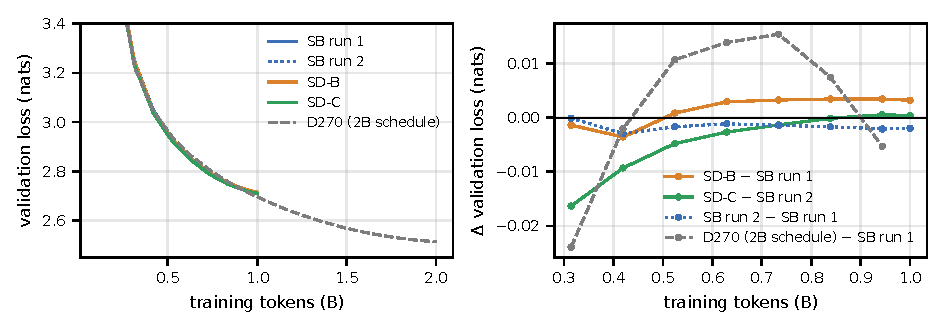
\includegraphics[width=\textwidth]{figures/loss_curves.pdf}
\caption{Validation loss vs.\ training tokens (left) and differences (right). The two \SB{} runs (dotted) define the
noise floor. \Dense{} follows a 2B-token schedule, so at equal tokens its learning rate is still higher.}
\label{fig:loss}
\end{figure*}

\begin{table}[t]
\centering
\small
\begin{tabular}{lrr}
\toprule
model & val loss & $\Delta$ vs.\ matched \SB{} \\
\midrule
\SB{} run 1 & 2.7127 & -- \\
\SB{} run 2 & 2.7107 & $-0.0020$ (replicate) \\
\SDB & 2.7159 & $+0.0032$ \\
\SDC & 2.7111 & $+0.0004$ \\
\bottomrule
\end{tabular}
\caption{Validation loss (nats) after 1B tokens.}
\label{tab:loss}
\end{table}

Both self-drafting models finish within noise of the baseline (Table~\ref{tab:loss}, Figure~\ref{fig:loss}): $+0.0032$
for \SDB{} and $+0.0004$ for \SDC, against a replicate difference of $0.0020$. In other words, neither replacing the
hidden-state router with a token-only one nor adding a distillation loss on the memory degrades language modelling.
\SDB{} shows a reproducible gradient-norm spike at step 20 that recovers by step 30. No run had a non-finite loss.

The same holds downstream. On zero-shot HellaSwag \citep{zellers2019hellaswag}, cloze MMLU \citep{hendrycks2021mmlu}, SciQ
\citep{welbl2017sciq}, WinoGrande \citep{sakaguchi2020winogrande}, PIQA \citep{bisk2020piqa} and ARC-Easy
\citep{clark2018arc}, evaluated with lm-eval \citep{gao2023lmeval}, no paired difference between a self-drafting model
and \SB{} excludes zero (Table~\ref{tab:lmeval}).

\begin{table}[t]
\centering
\small
\setlength{\tabcolsep}{2.6pt}
\begin{tabular}{lcccccc}
\toprule
 & HS & MMLU & SciQ & WG & PIQA & ARC-E \\
\midrule
\SB{} run 1 & 28.7 & 24.7 & 60.1 & 51.7 & 58.9 & 38.9 \\
\SB{} run 2 & 29.3 & 24.6 & 60.4 & 51.8 & 60.0 & 38.0 \\
\SDB & 28.6 & 24.7 & 58.6 & 50.4 & 59.7 & 39.0 \\
\SDC & 28.6 & 24.3 & 60.3 & 51.6 & 58.3 & 40.0 \\
\midrule
\SDB$-$\SB & $-0.1$ & $0.0$ & $-1.5$ & $-1.3$ & $+0.8$ & $0.0$ \\
\SDC$-$\SB & $-0.1$ & $-0.4$ & $+0.2$ & $-0.1$ & $-0.7$ & $+1.1$ \\
\bottomrule
\end{tabular}
\caption{Zero-shot accuracy (\%). acc\_norm is used for HS, SciQ, PIQA and ARC-E; acc for MMLU-cloze and WG. No
self-drafting difference excludes 0 at 95\% (paired bootstrap; Appendix~\ref{app:lmeval}).}
\label{tab:lmeval}
\end{table}

%=====================================================================
\section{RQ2: Why it is free: codes are nearly token-determined}
\label{sec:why}
%=====================================================================

We dump every model's memory codes on the 1.54M held-out positions. We then predict each route's code from tokens alone,
fitting on 500 documents and evaluating on the other 500 (Table~\ref{tab:rq2}, Figure~\ref{fig:rq2}).

\begin{table}[t]
\centering
\small
\setlength{\tabcolsep}{3pt}
\begin{tabular}{lccc}
\toprule
predictor & \SB{} (hidden) & \SDB{} (embed2) & \SDC{} (+SSM) \\
\midrule
$x_t$ & \textbf{0.857} & 0.580 & 0.545 \\
$(x_{t-1},x_t)$ & 0.868 & 0.742 & 0.632 \\
MLP $x_{t-2..t}$ & 0.878 & 0.826 & 0.735 \\
\midrule
MLP top-1 code acc. & 0.881 & 0.834 & 0.738 \\
next-code recall@8 & 0.738 & 0.722 & 0.770 \\
P(some route misses)@8 & 0.987 & 0.989 & 0.988 \\
\bottomrule
\end{tabular}
\caption{Fraction of code entropy explained, $1-\mathrm{CE}/H(C)$, on held-out text (mean over routes; CIs
$\le\pm0.005$). The last two rows predict $c[t{+}1]$ from $(c[t-1],c[t])$.}
\label{tab:rq2}
\end{table}

\begin{figure}[t]
\centering
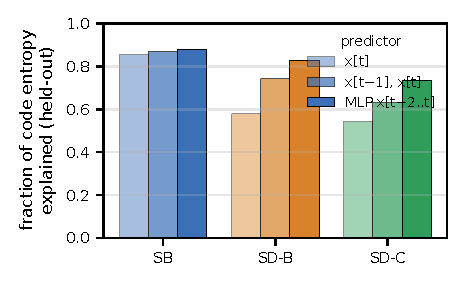
\includegraphics[width=\columnwidth]{figures/predictability.pdf}
\caption{Fraction of code entropy explained by token-only predictors.}
\label{fig:rq2}
\end{figure}

\SB's router reads the hidden state of block~1, yet the \emph{current token alone} explains 86\% of its code entropy, with
89.5\% top-1 accuracy per route. At layer~1 the hidden state carries little beyond the token itself, so the router has
learned what is effectively a token hash. \SDB's codes are an exact function of $(x_{t-1},x_t)$. Its count-table
scores are lower bounds, limited by bigram sparsity in the fitting half. \SDC's SSM deliberately injects document
context. The \emph{next} step's codes, in contrast, are unpredictable from the current codes: even with eight guesses per
route, at least one of 184 routes misses 98.7\% of the time. Prefetching must therefore stage all 16 candidates.

\paragraph{Substitution.}
Table~\ref{tab:subst} replaces \SB's codes at inference time. The memory is worth 0.28 nats, and codes predicted from three
tokens by a small MLP keep \textbf{99.8\%} of that value, even though they are only 88\% correct per route. Token-only
routing therefore costs nothing because \SB{} was, functionally, already routing on tokens.

\begin{table}[t]
\centering
\small
\begin{tabular}{lrr}
\toprule
codes fed to \SB's memory & val loss & $\Delta$ \\
\midrule
own (hidden-state router) & 2.7347 & -- \\
predicted from $x_{t-2..t}$ & 2.7353 & $+0.0006$ \\
memory output zeroed & 3.0180 & $+0.283$ \\
uniformly random codes & 3.0500 & $+0.315$ \\
\bottomrule
\end{tabular}
\caption{Code substitution on 1.54M held-out tokens.}
\label{tab:subst}
\end{table}

%=====================================================================
\section{RQ3: How well can the memory draft?}
\label{sec:drafting}
%=====================================================================

\paragraph{Decodability ladder.}
We score increasingly powerful decoders against the target's own argmax (Figure~\ref{fig:ladder}). The levels are:
counts of next tokens per memory row (with two controls, keyed by token $n$-grams or by codes from a random router); the
rows read with a zero query; a trained draft head; and a tuned lens
\citep{belrose2023tuned,nostalgebraist2020logitlens} after the memory block.

\begin{figure}[t]
\centering
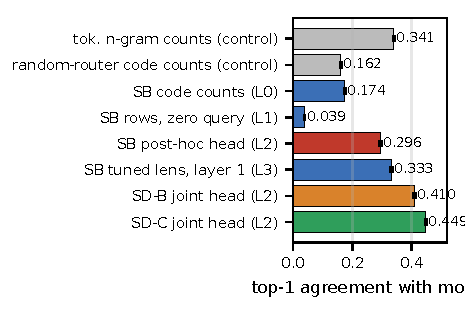
\includegraphics[width=\columnwidth]{figures/ladder.pdf}
\caption{Decodability ladder: top-1 agreement with the model's argmax on 1.54M held-out positions (95\% CIs).}
\label{fig:ladder}
\end{figure}

Static code statistics make a poor key: counts keyed by \SB's codes (0.174) barely beat a random router's (0.162) and
reach half the accuracy of plain token $n$-grams (0.341). A \emph{trained} readout over the same rows does far better.
\SB's post-hoc head reaches 0.296, which is 89\% of a tuned lens over the whole first layer (0.333). \textbf{Joint
training} lifts the memory-only decoder above both baselines, to 0.410 for \SDB{} and \textbf{0.449} for \SDC. The joint
heads overtake the post-hoc drafters early in training and stay ahead (Figure~\ref{fig:drafttrain}).

\begin{figure}[t]
\centering
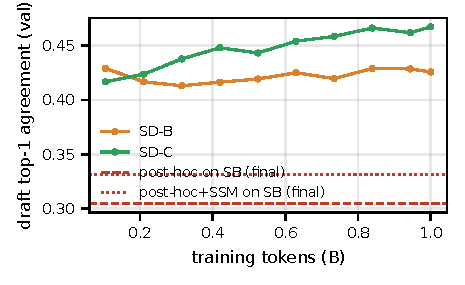
\includegraphics[width=\columnwidth]{figures/draft_training.pdf}
\caption{Draft-head top-1 agreement on validation during joint training. Horizontal lines show the final post-hoc
drafters fitted to the frozen baseline with 200M tokens.}
\label{fig:drafttrain}
\end{figure}

\paragraph{Offline acceptance.}
Table~\ref{tab:accept} and Figure~\ref{fig:accept} report accepted tokens per verification step at $\gamma{=}4$, on each
target's own greedy continuations. Drafted positions use codes the drafter computes itself, and online counts use only
verified text.

\begin{figure*}[t]
\centering
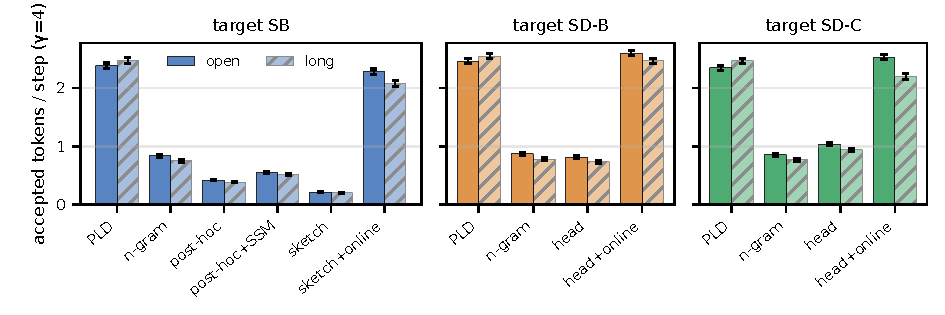
\includegraphics[width=\textwidth]{figures/acceptance.pdf}
\caption{Accepted tokens per verification step ($\gamma{=}4$) on open (solid) and long (hatched) prompts; 1{,}000
prompts each, 95\% CIs.}
\label{fig:accept}
\end{figure*}

\begin{table}[t]
\centering
\small
\setlength{\tabcolsep}{3pt}
\begin{tabular}{llcc}
\toprule
target & drafter & open & long \\
\midrule
\multirow{6}{*}{\SB} & \PLD{} \citep{saxena2023pld} & 2.38 & 2.47 \\
 & token $n$-gram (300M tok.) & 0.84 & 0.75 \\
 & post-hoc head & 0.42 & 0.39 \\
 & post-hoc head + SSM & 0.55 & 0.51 \\
 & sketch & 0.21 & 0.21 \\
 & sketch + online & 2.28 & 2.07 \\
\midrule
\multirow{3}{*}{\SDB} & \PLD & 2.46 & \textbf{2.54} \\
 & joint head & 0.81 & 0.73 \\
 & joint head + online & \textbf{2.59} & 2.46 \\
\midrule
\multirow{3}{*}{\SDC} & \PLD & 2.34 & \textbf{2.46} \\
 & joint head & \textbf{1.04} & \textbf{0.94} \\
 & joint head + online & \textbf{2.52} & 2.19 \\
\bottomrule
\end{tabular}
\caption{Mean accepted tokens per step at $\gamma{=}4$ (CIs $\le\pm0.06$). The token $n$-gram baseline scores
0.86--0.87 (open) and 0.77--0.78 (long) on \SDB{} and \SDC. Appendix~\ref{app:accept} has all $\gamma$.}
\label{tab:accept}
\end{table}

\emph{Joint beats post-hoc.} Without online counts, the joint heads accept 0.81--1.04 tokens per step, about twice the
post-hoc heads (0.42--0.55). \SDC's head is the only memory-only drafter that beats the token $n$-gram baseline (1.04 vs.\
0.86). Document context helps twice. In the post-hoc pair, adding the SSM improves acceptance by $+32.3\%$ (CI
$[+29.4,+35.2]\%$) on long text, which motivated \SDC. In the joint heads, \SDC{} improves on \SDB{} by $+27$--$28\%$.

\emph{Online counts are the large lever.} Adding code-keyed counts from verified text lifts the heads to 2.5--2.6 tokens
per step. Paired on the same continuations, this is better than \PLD{} on open text ($+0.13\ci{+0.12}{+0.15}$ for \SDB,
$+0.18\ci{+0.17}{+0.20}$ for \SDC) and below it on long documents ($-0.08$, $-0.27$). Most of this gain is available to an
unmodified memory model as well: \SB{} with a static sketch and online counts reaches 2.28. The jointly trained head
contributes the remaining ${\sim}0.3$ tokens per step.

%=====================================================================
\section{RQ4a: When does self-drafting help?}
\label{sec:when}
%=====================================================================

\paragraph{Prompt lookup harvests greedy self-repetition.}
We measure how much of each greedy continuation repeats a 5-gram that appeared earlier (Table~\ref{tab:repeat}).
59--62\% of continuation tokens do so. Only 10--16\% copy the \emph{prompt}; about 49\% copy the model's \emph{own} earlier
output. The copied fraction climbs from 9--16\% in the first 16 tokens to 87--92\% in the last 32: greedy continuations of
these models degenerate into loops, and exact-match lookup exploits them.

\begin{table}[t]
\centering
\small
\setlength{\tabcolsep}{3pt}
\begin{tabular}{lccc}
\toprule
 & \SB & \SDB & \SDC \\
\midrule
copied (any source), open & 0.60 & 0.62 & 0.59 \\
\quad from the prompt & 0.10 & 0.12 & 0.10 \\
\quad from own continuation & 0.49 & 0.50 & 0.49 \\
first 16 tokens & 0.10 & 0.10 & 0.09 \\
last 32 tokens & 0.87 & 0.90 & 0.87 \\
\bottomrule
\end{tabular}
\caption{Fraction of greedy continuation tokens that repeat an earlier 5-gram (open prompts).}
\label{tab:repeat}
\end{table}

\paragraph{Learned drafters win before repetition sets in.}
Figure~\ref{fig:continuation} plots acceptance along the continuation. In the first 16 tokens, \PLD{} accepts only 0.65
tokens per step on open text. The self-drafting heads accept 0.92 (\SDC) and 0.80 (\SDB) on their own, and
\textbf{1.07 and 1.06} with online counts: \textbf{40--65\% more than prompt lookup}. \PLD{} overtakes them only as the
loop forms, reaching 3.26 by the end. The headline acceptance numbers of every drafter are thus dominated by a degenerate
regime that sampled decoding and larger models largely avoid. In the regime that matters for less repetitive text, the
self-drafting memory is the stronger drafter.

\begin{figure*}[t]
\centering
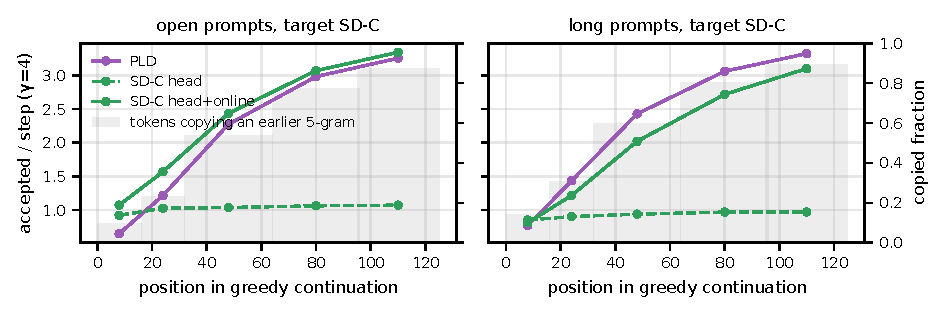
\includegraphics[width=\textwidth]{figures/continuation.pdf}
\caption{Accepted tokens per step ($\gamma{=}4$) along the 128-token greedy continuation (\SDC; open and long prompts).
Grey bars: fraction of continuation tokens that repeat an earlier 5-gram.}
\label{fig:continuation}
\end{figure*}

\paragraph{A hybrid drafter beats prompt lookup.}
\PLD{} finds a match on 89--96\% of rows. Using it when it matches, and the self-drafting head otherwise, beats \PLD{} on
every target and text type (Table~\ref{tab:hybrid}): $+0.11$ to $+0.13$ tokens per step on open text and $+0.05$ to
$+0.06$ on long text, with every CI excluding zero. Where \PLD{} has no match, \SDC's head accepts 1.24 tokens. A token
$n$-gram fills the same gaps nearly as well (within 0.01 overall). A per-row oracle between the two drafters reaches
2.70--2.75, about $+0.3$ tokens per step above \PLD. The remaining headroom therefore lies in \emph{deciding which drafter
to trust}, which the next finding addresses.

\begin{table}[t]
\centering
\small
\setlength{\tabcolsep}{2.5pt}
\begin{tabular}{llcccc}
\toprule
target & text & \PLD & hybrid & $\Delta$ (95\% CI) & oracle \\
\midrule
\SDC & open & 2.341 & 2.471 & $+0.130\ci{0.123}{0.138}$ & 2.700 \\
\SDC & long & 2.460 & 2.516 & $+0.057\ci{0.052}{0.061}$ & 2.747 \\
\SDB & open & 2.458 & 2.569 & $+0.111\ci{0.104}{0.118}$ & 2.737 \\
\SDB & long & 2.541 & 2.587 & $+0.045\ci{0.042}{0.049}$ & 2.753 \\
\bottomrule
\end{tabular}
\caption{Hybrid drafter (prompt lookup if it matches, else the self-drafting head) vs.\ prompt lookup alone, $\gamma{=}4$.
The oracle takes the better of the two per row and is not deployable.}
\label{tab:hybrid}
\end{table}

\paragraph{The drafter knows when it is right.}
Draft agreement tracks the target's confidence. For \SDC{}, it is 23\% when the target's top probability is below 0.2 and
77\% above 0.9; across the third of positions where the target is confident ($>0.6$), it is 66\%. More usefully, the
drafter's \emph{own} confidence, available live without consulting the target, is informative and conservative.
Agreement exceeds the drafter's stated probability at every level: 61\% at 0.3--0.5 and 98\% above 0.9 (correlation
$0.50$; Figure~\ref{fig:confidence}). Drafting only when the drafter is at least 30\% confident covers 35\% of positions at
75\% agreement. At a 50\% threshold, it covers 18\% at \textbf{88\%}, against 45\% agreement unconditionally. This is the
signal needed for confidence-gated, adaptive-length drafting, and for a learned hybrid switch.

\begin{figure}[t]
\centering
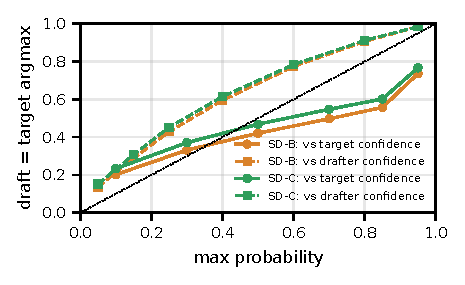
\includegraphics[width=\columnwidth]{figures/confidence.pdf}
\caption{Draft-head agreement with the target vs.\ the target's confidence (solid) and the drafter's own confidence
(dashed). Above the diagonal means the drafter is right more often than it claims.}
\label{fig:confidence}
\end{figure}

%=====================================================================
\section{RQ4b: What does the memory learn?}
\label{sec:learn}
%=====================================================================

\paragraph{Codes form emergent word classes.}
Without supervision, \SB's codes sort tokens into recognisable classes. Table~\ref{tab:pos} shows the route whose codes
carry the most information about coarse token type: it separates prepositions and conjunctions, determiners, subjects,
copulas and auxiliaries, possessives, and sentence-final punctuation. On average, a code carries 31\% of the token-class
entropy in \SB{} (43\% for the best route), against 22\% and 21\% for the token-only routers of \SDB{} and \SDC. Their codes
also mix in the previous token or document context.

\begin{table}[t]
\centering
\small
\setlength{\tabcolsep}{3pt}
\begin{tabular}{rrl}
\toprule
code & share & most frequent tokens \\
\midrule
12 & 13.5\% & \texttt{of to and in for with as on} \\
7 & 10.1\% & \texttt{the a The an this your A} \\
2 & 10.0\% & \texttt{it they cancer people It he there} \\
4 & 6.1\% & \texttt{is are was can and were more} \\
6 & 7.2\% & \texttt{you be I not also one all some} \\
5 & 3.8\% & \texttt{'s your " their his her these} \\
15 & 5.2\% & \texttt{. ? ) ). ! ."} \\
13 & 5.2\% & \texttt{\textbackslash n ( : " per} \\
\bottomrule
\end{tabular}
\caption{Emergent token classes in one \SB{} route (held-out text).}
\label{tab:pos}
\end{table}

\paragraph{Codes are not identifiable.}
The two \SB{} runs share initialisation and data order. They reach the same loss (2.7127 vs.\ 2.7107) and the same
downstream accuracy, yet assign the same code at a position only 36.8\% of the time (per route 19--53\%; chance 6.3\%).
Per-bit agreement is 77\%, and no position has all 184 routes identical. Many code assignments work equally well: the
memory needs a good token partition, not a particular one. Statements about individual codes describe one such solution.

\paragraph{The table is fully used, but hidden-state routes are redundant.}
Every row is addressed on held-out text (100\% of 2-gram rows, over 99.9\% of 3-gram rows), and usage is near-uniform.
The effective number of rows is 77\% (2-gram) and 61\% (3-gram) of the table for \SB, and the busiest 1\% of rows receive
only 5--9\% of hits. Capacity is not lost to dead rows but to \emph{duplicated} information (Figure~\ref{fig:redundancy}).
The mean normalised mutual information between two \SB{} routes is 0.231, against 0.087 (\SDB) and 0.085 (\SDC).
Because hidden-state routes all mostly re-encode the current token, \SB's 184 routes store overlapping views of one
partition. Token-only routing makes routes 2.7$\times$ more independent at no loss cost, a side benefit of
self-drafting.

\begin{figure}[t]
\centering
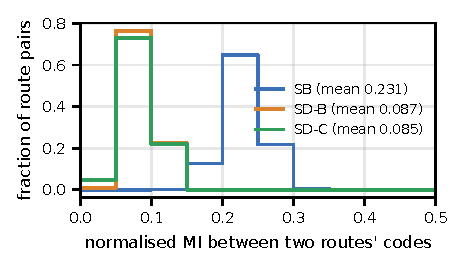
\includegraphics[width=\columnwidth]{figures/redundancy.pdf}
\caption{Pairwise normalised mutual information between routes' codes (3{,}000 random pairs).}
\label{fig:redundancy}
\end{figure}

\paragraph{The memory specialises in frequent, local and formatting tokens.}
Zeroing \SB's memory costs $0.283\ci{0.279}{0.288}$ nats, and the benefit is concentrated: the top 10\% of tokens account
for 72\% of it. It \emph{grows} with the frequency of the current token, from 0.15 nats (100--1K training occurrences) to
0.34 ($>$1M), counter to the view of memory as a store of rare facts. It is largest when predicting whitespace and newlines
(0.73), digits (0.35) and word continuations (0.32), and at the start of a window (0.37 nats at position 1, 0.28 beyond
512), where attention has little context. \SDC's memory is worth 0.216 nats at equal loss, so with token-only routing
the backbone takes on more of the work. Figure~\ref{fig:tokentypes} compares this with \Dense. With twice the training
tokens, the dense model is $0.18$ nats better overall, but only 0.035 better on whitespace and 0.089 on punctuation,
against 0.21 on word starts. Draft agreement follows the same pattern: 83\% on whitespace, 55\% on punctuation, 21\% on
digits. Where the memory works hardest, it nearly matches a dense model trained on twice the data, and it drafts best.

\begin{figure*}[t]
\centering
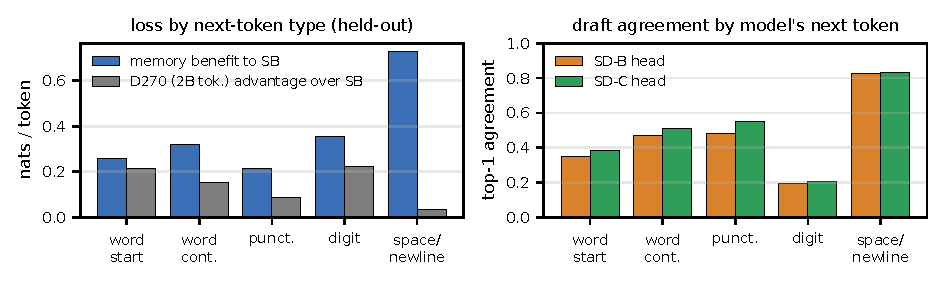
\includegraphics[width=\textwidth]{figures/token_types.pdf}
\caption{Left: per-token loss reduction from \SB's memory, and the 2B-token dense model's remaining advantage, by type of
the token being predicted. Right: draft-head agreement with the target by the target's predicted token type.}
\label{fig:tokentypes}
\end{figure*}

\paragraph{Is the table worth having at this scale?}
At equal training tokens, \Dense{} matches \SB{}: 2.7167 vs.\ 2.7220 at 0.94B tokens, while still on a higher learning
rate. Together with the redundancy and specialisation results, this suggests that at 370M parameters the table mostly
re-encodes local token statistics that a dense model of equal active size also learns. Memory layers have been reported to pay off at
larger scale \citep{berges2024memory}, and route decorrelation (above) is a direct lever we have not yet tested.

%=====================================================================
\section{Serving and speed}
\label{sec:serving}
%=====================================================================

\paragraph{Exactness.}
B0, B1 and B4 produce identical tokens and bitwise-identical logits in fp32 and fp16, for \SDC{} and \SB{} (100 prompts
$\times$ 128 tokens). Our C++ CPU drafter matches the PyTorch reference on 10k positions: identical codes and shortlists,
$|\Delta\text{logit}|\le9.5\times10^{-6}$, and argmax agreement 1.0. Live speculative decoding reproduces greedy output
exactly in fp32. In fp16 it matches 89--91\% of prompts, and every mismatch is a near-tie (top-2 margin $<10^{-2}$).

\paragraph{Host-memory serving.}
With \SDC's 0.2\,GB table, a decode step takes 25.3/25.7/25.7\,ms (B0/B1/B4) at batch 1 and 26.7/26.6/26.9\,ms at batch 16.
Serving from host RAM thus costs ${\approx}1\%$, and the synchronous gather (93\,KB per token) already hides it. Step latency
is flat from batch 1 to 16, so verifying $\gamma{+}1$ tokens costs about one step, which supports the speedup model.

\paragraph{Speedup model and live status.}
Combining offline acceptance with the measured cost of the PyTorch drafter (1.3\,ms per token, $c=0.059$), the \SDC{}
head with online counts gives an implied \textbf{2.86$\times$} speedup on open text at $\gamma{=}4$ (2.59$\times$ long),
and 3.30$\times$ at $\gamma{=}6$ (Figure~\ref{fig:speedup}). Our first live implementation does not yet realise this. With
a single-threaded C++ drafter (10.3\,ms per token, 3.6\,ms on 4 threads), no online counts, and a sketch-based shortlist
that lowers acceptance to 0.53--0.63, the loop runs at 0.49$\times$ ($\gamma{=}2$) and 0.28$\times$ ($\gamma{=}4$) of
greedy speed, with the GPU idle 86--92\% of the time. Each cause is an engineering issue, listed in \S\ref{sec:future}.

\begin{figure*}[t]
\centering
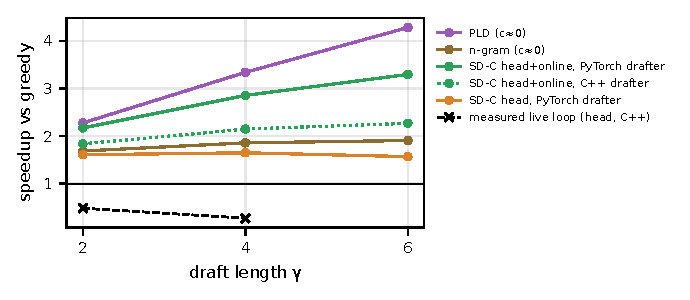
\includegraphics[width=0.72\textwidth]{figures/speedup.pdf}
\caption{Implied speedup $\mathbb{E}[A{+}1]/(1+\gamma c)$ on open text for \SDC{} with measured drafter costs, with the
current live implementation for reference.}
\label{fig:speedup}
\end{figure*}

%=====================================================================
\section{Directions the evidence supports}
\label{sec:future}
%=====================================================================

\begin{enumerate}
\setlength\itemsep{1pt}
\item \textbf{Evaluate outside the degenerate regime.} Half of all greedy continuation tokens are self-copies. Sampling,
repetition penalties, instruction-following prompts and larger targets move decoding toward the early-continuation
regime, where self-drafting heads beat prompt lookup by 40--65\%.
\item \textbf{Learn the switch.} A per-row oracle between prompt lookup and the head is worth $\approx\!+0.3$ tokens per
step. The drafter's own confidence, \PLD's match length and the predicted token type are all available live, and all are
predictive.
\item \textbf{Confidence-gated, adaptive-length drafting.} At a 0.5 threshold the drafter is right 88\% of the time.
Drafting long blocks only when confident would cut wasted verification.
\item \textbf{Decorrelate routes.} Hidden-state routes are 2.7$\times$ more redundant than token-routed ones. Diversity
objectives, or token-only routing at fixed parameters, could convert duplicated capacity into new capacity. That is the
direct test of whether the table can beat an iso-active dense model.
\item \textbf{Specialise the memory.} Its benefit concentrates on frequent, local and formatting tokens. Routing only
those tokens through the table, or sizing the table for that role, would spend parameters where they help.
\item \textbf{Realise the speedup.} Move online counts into the C++ loop, optimise the drafter (the PyTorch reference is
already 8$\times$ faster), and use the head rather than a sketch to form the shortlist. Staging exact rows for drafted blocks
is already supported by the serving layer.
\item \textbf{Scale.} The drafter never runs the backbone, so its cost relative to the target falls with model size. Testing
whether acceptance holds against 1--7B targets is the key next experiment.
\end{enumerate}

%=====================================================================
\section{Related Work}
\label{sec:related}
%=====================================================================

\paragraph{Drafters.}
Drafters include separate small models \citep{leviathan2023fast,chen2023accelerating}, distilled drafters
\citep{zhou2024distillspec}, heads on the target's hidden states \citep{stern2018blockwise,cai2024medusa,li2024eagle},
and model-free retrieval from the prompt or a datastore \citep{saxena2023pld,he2024rest,fu2024lookahead}. A self-drafting
memory sits in between. Like decoding heads, it is trained with the target. Like retrieval, it never runs the backbone.
Our analysis of greedy self-repetition gives one explanation for why simple copying is so strong for small models, and
shows how learned and copying drafters complement each other.

\paragraph{Memory layers.}
Product-key memories \citep{lample2019pkm} and memory layers at scale \citep{berges2024memory} add sparse, high-capacity
parameters. Route $n$-gram memory \citep{lngram} addresses rows by quantised codes over a short window. To our knowledge,
this is the first study of whether such a memory can draft for its own model, how token-determined its addressing is, what
its codes encode, and how to serve it exactly from host memory \citep[cf.][]{sheng2023flexgen}.

\paragraph{Reading early predictions.}
Logit and tuned lenses \citep{nostalgebraist2020logitlens,belrose2023tuned} decode intermediate layers. We use them as an
upper reference for what the memory block carries, and find that a jointly trained memory-only head exceeds a tuned lens
over the whole first layer.

%=====================================================================
\section{Conclusion}
%=====================================================================

An $n$-gram memory can be made to draft for its own model at no cost to the model. Layer-1 routing is already almost a
per-token lookup, so token-only routing removes nothing the model relied on. A jointly trained head reading the memory
is a much better drafter than one fitted afterwards, document context helps it further, and code-keyed online counts make
it competitive with prompt lookup. Looking inside the models shows what the memory learns: a non-unique, word-class-like
partition that helps most on local and formatting tokens. It also shows when self-drafting helps: before greedy
decoding falls into the self-repetition that prompt lookup exploits, and in combination with it. Turning these gains into
wall-clock speed, and testing them at scale and under sampling, are the natural next steps.

%=====================================================================
\section*{Limitations}
%=====================================================================

\begin{itemize}
\setlength\itemsep{1pt}
\item \textbf{Scale and seeds.} All models have 370M parameters and are trained on 1B tokens (2B for \Dense). The
baseline was trained twice, and the other models once. Differences below about 0.003 nats or one accuracy point are not
resolvable.
\item \textbf{Decoding regime.} Acceptance is measured under greedy decoding, whose continuations are highly repetitive
(\S\ref{sec:when}). Results under sampling are untested.
\item \textbf{Speed.} Speedups are modelled from offline acceptance and measured component costs. The current live
implementation is slower than greedy decoding (\S\ref{sec:serving}).
\item \textbf{Missing controls.} We did not run: a dense model on the same 1B-token schedule; online counts keyed by token
$n$-grams instead of codes; a draft head without the table; tables larger than GPU memory; or a code-domain text type.
\item \textbf{Interpretability.} Codes are not identifiable across runs, so per-code descriptions concern one solution.
Token classes come from a heuristic over the tokenizer. The dense comparison by token type is budget-confounded. A count-based
estimate of next-token information carried by codes beyond the current token proved unreliable at our sample size and is
not reported.
\item \textbf{Held-out set.} Drafting and analysis use 1{,}000 long documents. Open prompts are their first 256 tokens.
\end{itemize}

\section*{Ethics Statement}
We train small language models on a public web corpus \citep{diao2025climb} and evaluate them on public benchmarks.
The models are not deployed. The work targets more efficient inference and carries the usual dual-use considerations of
language-model research. We release code, configurations, logs and results so that every reported number can be traced.

\bibliography{references}

\appendix

%=====================================================================
\section{Training and compute details}
\label{app:train}
%=====================================================================

\begin{table}[h]
\centering
\small
\setlength{\tabcolsep}{3pt}
\begin{tabular}{lllrr}
\toprule
run & GPUs & micro-batch & tok/s & hours \\
\midrule
\SB{} run 1 & 4$\times$RTX 2080 Ti & 2 & 20.5K & 14.8 \\
\SDB & 4$\times$RTX 2080 Ti & 1 & 17.2K & 17.4 \\
\Dense{} (2B) & 4$\times$RTX 2080 Ti & 2 & 29.2K & 20.8 \\
\SB{} run 2 & 2$\times$V100 & 4 & 12.9K & 22.4 \\
\SDC & 2$\times$V100 & 2 & 12.3K & 23.6 \\
post-hoc drafters & 1$\times$RTX 2080 Ti each & 4 & -- & -- \\
\bottomrule
\end{tabular}
\caption{Compute per run. The global batch ($256\times2048$), schedule and data order are identical across runs. Only the
micro-batch (and hence the number of gradient-accumulation steps) differs, chosen to fit GPU memory; 4-GPU runs shard optimizer state with ZeRO-1 \citep{rajbhandari2020zero}. \SDB{} is compared
with \SB{} run 1 and \SDC{} with \SB{} run 2. Analyses and offline evaluation used one RTX 5070 Laptop GPU. Serving, drafter
and lm-eval measurements used one V100.}
\end{table}

\paragraph{Memory configuration.}
Following the reference initialisation, tables are $\mathcal{N}(0,0.02^2)$ and the readout output projection is
zero-initialised, so the memory starts as the identity. The short convolution (kernel 4, dilation 3) is zero-initialised,
the surrogate is approximate, and the router runs in fp32. The readout has 16 query and 4 KV heads of dimension 64, with sink
mass $m=0.5$. At the end of training, routes use 14.7 (\SB), 14.6 (\SDB) and 13.4 (\SDC) effective codes out of 16, with
no dead codes, and the sink takes 0.39--0.40 of the attention mass.

\paragraph{Draft loss and post-hoc drafter.}
$\lambda=0.1$ on 25\% of positions, 512-position chunks, fp32 KL. In final validation, draft KL is 1.67 (\SDB) and 1.44
(\SDC). The post-hoc router imitation reaches 93.8\% bit accuracy and 78.9\% code accuracy per route, with validation KL
2.61 (2.30 with the SSM).

%=====================================================================
\section{Full lm-eval results}
\label{app:lmeval}
%=====================================================================

\begin{table*}[t]
\centering
\small
\begin{tabular}{lcccccc}
\toprule
$a-b$ (points) & HellaSwag & MMLU-cloze & SciQ & WinoGrande & PIQA & ARC-E \\
\midrule
\SDB{} $-$ \SB & $-0.1\ci{-0.7}{+0.4}$ & $-0.0\ci{-0.5}{+0.5}$ & $-1.5\ci{-3.7}{+0.7}$ & $-1.3\ci{-4.6}{+2.1}$ & $+0.8\ci{-0.9}{+2.3}$ & $+0.0\ci{-1.4}{+1.5}$ \\
\SDC{} $-$ \SB & $-0.1\ci{-0.7}{+0.4}$ & $-0.4\ci{-0.9}{+0.1}$ & $+0.2\ci{-2.1}{+2.5}$ & $-0.1\ci{-3.4}{+3.4}$ & $-0.7\ci{-2.2}{+0.9}$ & $+1.1\ci{-0.4}{+2.5}$ \\
\SDC{} $-$ \SDB & $-0.0\ci{-0.6}{+0.6}$ & $-0.4\ci{-0.9}{+0.2}$ & $+1.7\ci{-0.3}{+3.8}$ & $+1.2\ci{-2.1}{+4.3}$ & $-1.4\ci{-3.0}{+0.1}$ & $+1.0\ci{-0.5}{+2.5}$ \\
\SB{} run 2 $-$ run 1 & $+0.6\ci{+0.0}{+1.2}$ & $-0.1\ci{-0.6}{+0.4}$ & $+0.3\ci{-1.9}{+2.5}$ & $+0.1\ci{-3.2}{+3.3}$ & $+1.0\ci{-0.5}{+2.6}$ & $-0.9\ci{-2.3}{+0.5}$ \\
\Dense{} $-$ \SB & $+2.2\ci{+1.6}{+2.9}$ & $+0.3\ci{-0.2}{+0.9}$ & $+8.0\ci{+5.7}{+10.3}$ & $+0.9\ci{-2.6}{+4.4}$ & $+2.6\ci{+1.0}{+4.2}$ & $+2.2\ci{+0.7}{+3.8}$ \\
\bottomrule
\end{tabular}
\caption{Paired differences with 95\% bootstrap CIs (lm-eval 0.4.13, zero-shot; \texttt{mmlu\_continuation} pooled
over 57 subjects). \SB{} denotes run 1 unless stated. \Dense{} was trained on 2$\times$ the tokens.}
\end{table*}

%=====================================================================
\section{Full acceptance results}
\label{app:accept}
%=====================================================================

\begin{table*}[t]
\centering
\small
\setlength{\tabcolsep}{3pt}
\begin{tabular}{llcccccc}
\toprule
 & & \multicolumn{3}{c}{open} & \multicolumn{3}{c}{long} \\
target & drafter & $\gamma{=}2$ & $\gamma{=}4$ & $\gamma{=}6$ & $\gamma{=}2$ & $\gamma{=}4$ & $\gamma{=}6$ \\
\midrule
\SB & \PLD & 1.297 & 2.379 & 3.331 & 1.355 & 2.469 & 3.453 \\
\SB & token $n$-gram & 0.674 & 0.839 & 0.889 & 0.619 & 0.753 & 0.788 \\
\SB & post-hoc & 0.386 & 0.421 & 0.428 & 0.361 & 0.386 & 0.388 \\
\SB & post-hoc + SSM & 0.481 & 0.549 & 0.562 & 0.454 & 0.510 & 0.518 \\
\SB & sketch & 0.201 & 0.212 & 0.212 & 0.198 & 0.206 & 0.206 \\
\SB & sketch + online & 1.297 & 2.275 & 3.062 & 1.242 & 2.071 & 2.681 \\
\SDB & \PLD & 1.330 & 2.458 & 3.467 & 1.385 & 2.541 & 3.571 \\
\SDB & token $n$-gram & 0.692 & 0.868 & 0.922 & 0.634 & 0.777 & 0.816 \\
\SDB & joint head & 0.660 & 0.813 & 0.858 & 0.608 & 0.733 & 0.773 \\
\SDB & joint head + online & 1.451 & 2.591 & 3.567 & 1.394 & 2.460 & 3.343 \\
\SDC & \PLD & 1.277 & 2.341 & 3.282 & 1.348 & 2.460 & 3.445 \\
\SDC & token $n$-gram & 0.687 & 0.859 & 0.908 & 0.628 & 0.766 & 0.802 \\
\SDC & joint head & 0.797 & 1.036 & 1.120 & 0.739 & 0.939 & 1.000 \\
\SDC & joint head + online & 1.425 & 2.524 & 3.454 & 1.272 & 2.193 & 2.940 \\
\bottomrule
\end{tabular}
\caption{Mean accepted tokens per verification step on 1{,}000 prompts per text type.}
\end{table*}

%=====================================================================
\section{Reproducibility}
\label{app:repro}
%=====================================================================

The released repository contains the training stack and vendored \Lngram{} module, every configuration, the evaluation,
serving and interpretability code, all training logs (every logged step and evaluation), and every results file behind the
tables and figures. \texttt{paper/make\_figures.py} regenerates all figures from those files. 231 CPU unit tests cover
the claims the implementation relies on: bitwise backbone isolation of the draft path, stop-gradient destinations, scan
exactness, cached-decoding equivalence, serving-layout equivalence, and resume determinism.
\end{document}
